\begin{figure}[ht]
\centering
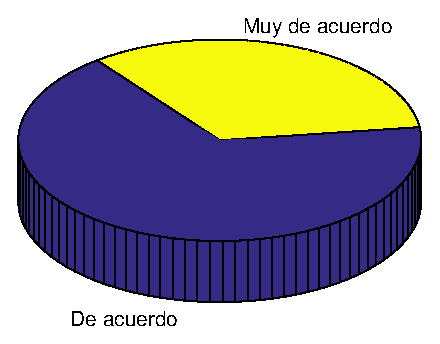
\includegraphics[width=0.5\columnwidth]{./figure/graph1.eps}
\caption{La normativa que regula el programa de postgrado es clara y conocida}
\label{graph1}
\end{figure}

\begin{figure}[ht]
\centering
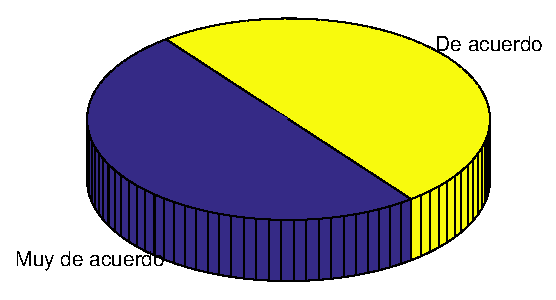
\includegraphics[width=0.5\columnwidth]{./figure/graph2.eps}
\caption{El plan de formación del programa es conocido por los académicos}
\label{graph2}
\end{figure}

\begin{figure}[ht]
\centering
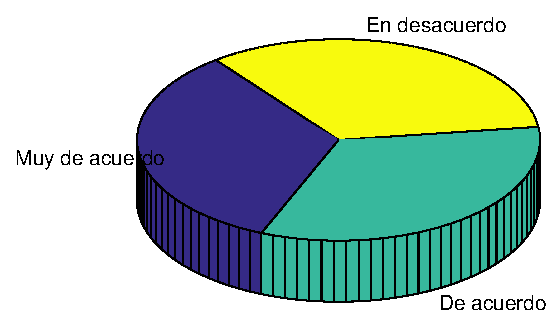
\includegraphics[width=0.5\columnwidth]{./figure/graph3.eps}
\caption{En general, el programa funciona de manera eficiente y ordenada en términos académicos}
\label{graph3}
\end{figure}

\begin{figure}[ht]
\centering
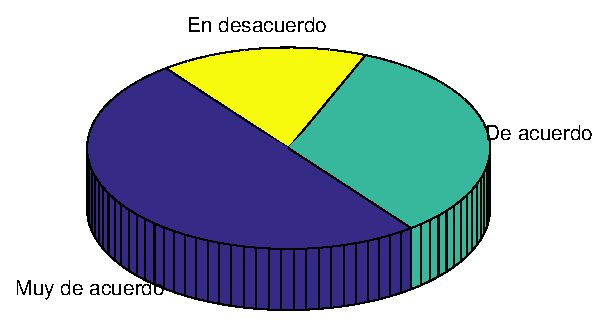
\includegraphics[width=0.5\columnwidth]{./figure/graph4.eps}
\caption{Cuando tengo un problema siempre recibo la orientación e información adecuada para resolverlo}
\label{graph4}
\end{figure}

\begin{figure}[ht]
\centering
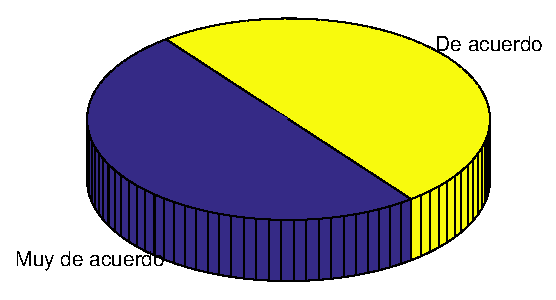
\includegraphics[width=0.5\columnwidth]{./figure/graph5.eps}
\caption{Existen actividades que permiten la coordinación entre los académicos del programa}
\label{graph5}
\end{figure}

\begin{figure}[ht]
\centering
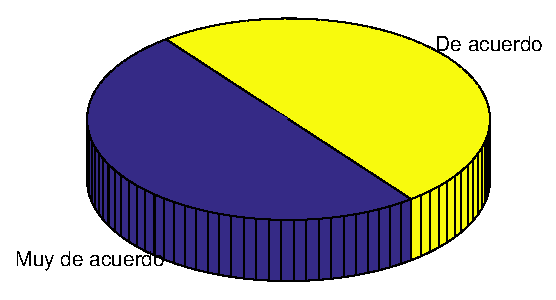
\includegraphics[width=0.5\columnwidth]{./figure/graph6.eps}
\caption{Existen instancias de participación de los académicos para la toma de decisiones en temas relevantes del programa (malla curricular, sistemas de evaluación, otros)}
\label{graph6}
\end{figure}

\begin{figure}[ht]
\centering
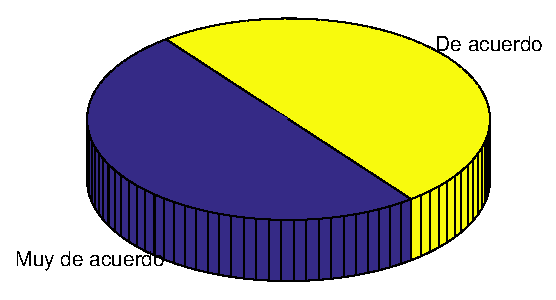
\includegraphics[width=0.5\columnwidth]{./figure/graph7.eps}
\caption{Los canales para comunicarse con los estudiantes son los adecuados}
\label{graph7}
\end{figure}

\begin{figure}[ht]
\centering
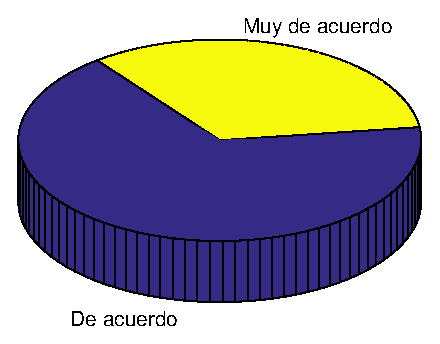
\includegraphics[width=0.5\columnwidth]{./figure/graph8.eps}
\caption{El programa tiene objetivos claros y conocidos}
\label{graph8}
\end{figure}

\begin{figure}[ht]
\centering
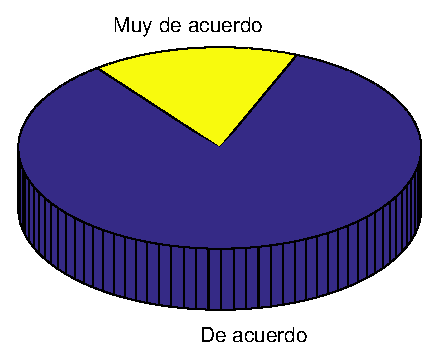
\includegraphics[width=0.5\columnwidth]{./figure/graph9.eps}
\caption{Los objetivos son congruentes con el enfoque del programa}
\label{graph9}
\end{figure}

\begin{figure}[ht]
\centering
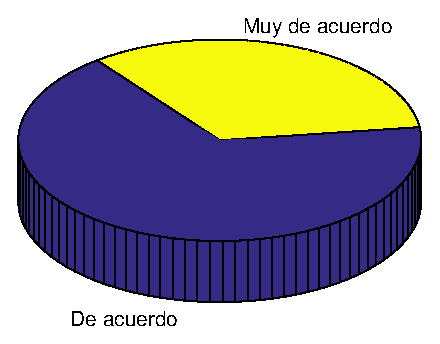
\includegraphics[width=0.5\columnwidth]{./figure/graph10.eps}
\caption{El perfil de graduación del programa es conocido por los académicos}
\label{graph10}
\end{figure}

\begin{figure}[ht]
\centering
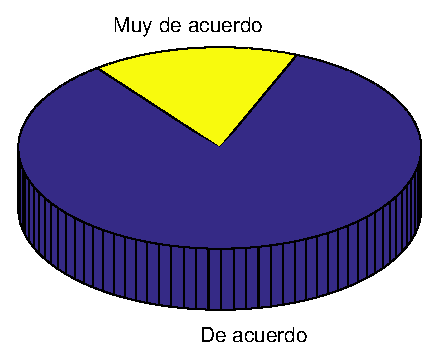
\includegraphics[width=0.5\columnwidth]{./figure/graph11.eps}
\caption{El programa tiene un perfil de graduación claro}
\label{graph11}
\end{figure}

\begin{figure}[ht]
\centering
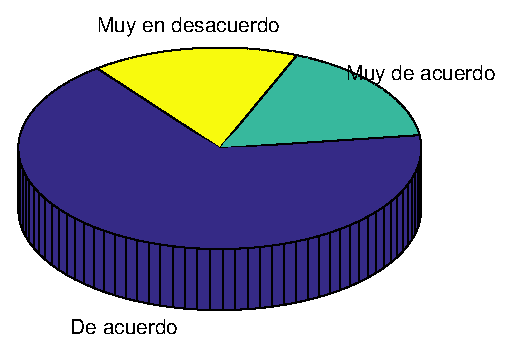
\includegraphics[width=0.5\columnwidth]{./figure/graph12.eps}
\caption{El perfil de egreso logra dar cuenta de los objetivos del programa}
\label{graph12}
\end{figure}

\begin{figure}[ht]
\centering
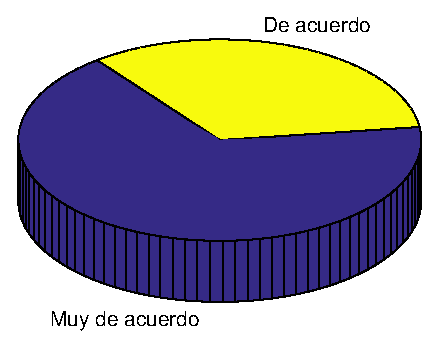
\includegraphics[width=0.5\columnwidth]{./figure/graph13.eps}
\caption{Los alumnos que ingresan al programa son acordes al perfil de egreso y las exigencias  del programa}
\label{graph13}
\end{figure}

\begin{figure}[ht]
\centering
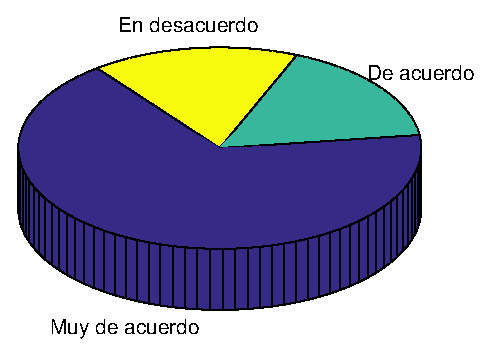
\includegraphics[width=0.5\columnwidth]{./figure/graph14.eps}
\caption{Los requisitos y criterios de admisión al programa son claros}
\label{graph14}
\end{figure}

\begin{figure}[ht]
\centering
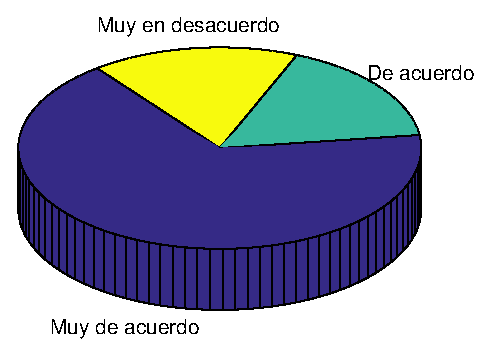
\includegraphics[width=0.5\columnwidth]{./figure/graph15.eps}
\caption{La periodicidad de las clases y el horario son adecuados para el cumplimiento de los objetivos del programa}
\label{graph15}
\end{figure}

\begin{figure}[ht]
\centering
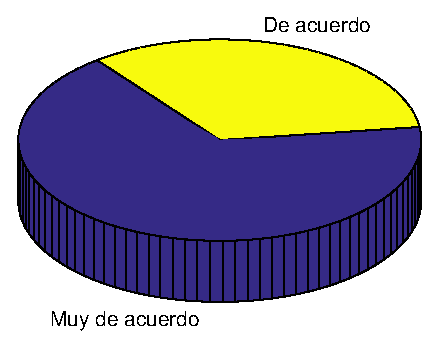
\includegraphics[width=0.5\columnwidth]{./figure/graph16.eps}
\caption{Los cursos y sus contenidos son pertinentes a las demandas actuales de la disciplina del programa}
\label{graph16}
\end{figure}

\begin{figure}[ht]
\centering
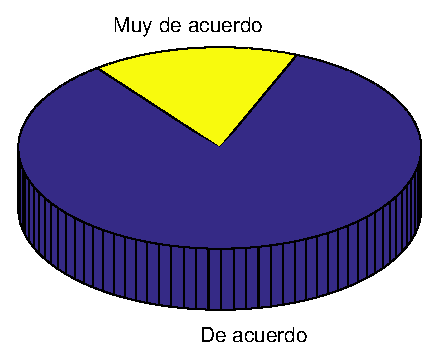
\includegraphics[width=0.5\columnwidth]{./figure/graph17.eps}
\caption{Los contenidos entregados en los distintos cursos se encuentran actualizados}
\label{graph17}
\end{figure}

\begin{figure}[ht]
\centering
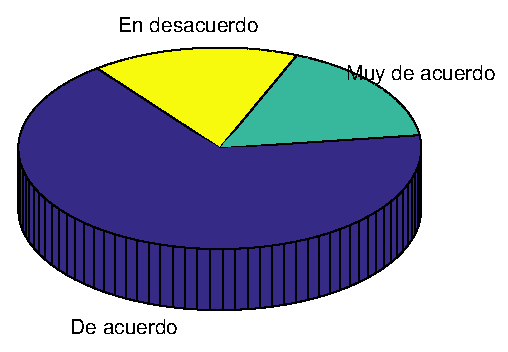
\includegraphics[width=0.5\columnwidth]{./figure/graph18.eps}
\caption{Las metodologías de enseñanza utilizadas por los profesores permiten alcanzar los objetivos propuestos en cada curso}
\label{graph18}
\end{figure}

\begin{figure}[ht]
\centering
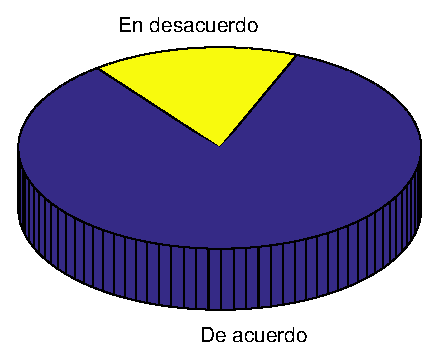
\includegraphics[width=0.5\columnwidth]{./figure/graph19.eps}
\caption{La forma de evaluación a los estudiantes está basada en criterios establecidos y difundidos al inicio de cada curso}
\label{graph19}
\end{figure}

\begin{figure}[ht]
\centering
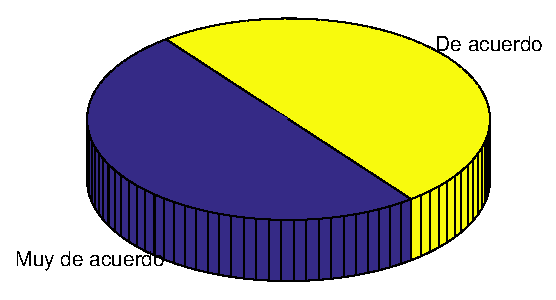
\includegraphics[width=0.5\columnwidth]{./figure/graph20.eps}
\caption{La forma de evaluación en los cursos promueven el aprendizaje de los contenidos}
\label{graph20}
\end{figure}

\begin{figure}[ht]
\centering
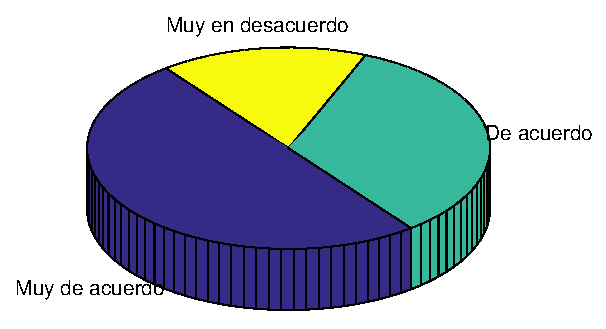
\includegraphics[width=0.5\columnwidth]{./figure/graph21.eps}
\caption{En los cursos se desarrollan actividades teóricas y prácticas}
\label{graph21}
\end{figure}

\begin{figure}[ht]
\centering
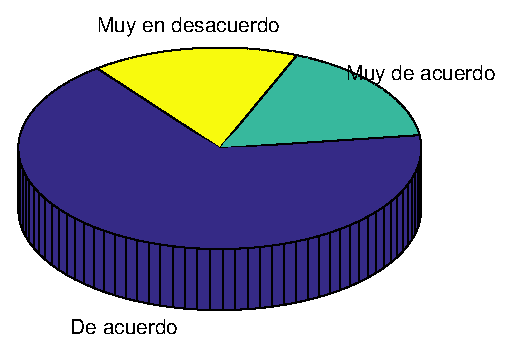
\includegraphics[width=0.5\columnwidth]{./figure/graph22.eps}
\caption{Los procesos de elaboración de tesis están reglamentadas y son conocidos de antemano}
\label{graph22}
\end{figure}

\begin{figure}[ht]
\centering
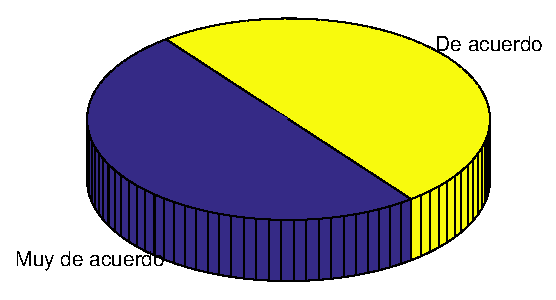
\includegraphics[width=0.5\columnwidth]{./figure/graph23.eps}
\caption{Las normas de graduación son conocidas y están claramente definidas}
\label{graph23}
\end{figure}

\begin{figure}[ht]
\centering
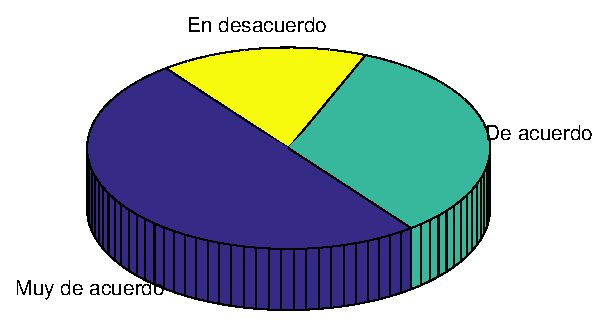
\includegraphics[width=0.5\columnwidth]{./figure/graph24.eps}
\caption{La actividad final de graduación responde adecuadamente al enfoque y perfil de graduación del programa}
\label{graph24}
\end{figure}

